\documentclass[10pt,a4paper]{article}
\usepackage[utf8]{inputenc}
\usepackage[T1]{fontenc,url}
\usepackage{multicol}
\usepackage{multirow}
\usepackage{parskip}
\usepackage{lmodern}
\usepackage{microtype}
\usepackage{verbatim}
\usepackage{amsmath, amssymb}
\usepackage{tikz}
\usepackage{physics}
\usepackage{mathtools}
\usepackage{algorithm}
\usepackage{algpseudocode}
\usepackage{listings}
\usepackage{enumerate}
\usepackage{enumitem}
\usepackage{graphicx}
\usepackage{float}
\usepackage{hyperref}
\usepackage{tabularx}
\usepackage{siunitx}
\usepackage{fancyvrb}
\usepackage{minted}
\usepackage{xcolor}
\usepackage[margin=2cm]{geometry}
\renewcommand{\baselinestretch}{1}
\renewcommand{\b}{\textbf}
\renewcommand{\exp}{e^}
\newcommand{\infint}{\int\limits_{-\infty}^{\infty}}
\newcommand{\limN}{\lim_{N\rightarrow \infty}}
\newcommand{\Gammaint}{\int\limits_{\Gamma_N}}

\usemintedstyle{pastie}

\begin{document}

\title{Home Exam - FYS3140}
\author{Candidate Number 15046}
\maketitle

\section*{Problem 1}
\begin{equation}
    y''(x) + \frac{3}{x}y'(x) - \frac{24}{x^2}y(x) = 56x^6
\end{equation}

\subsection*{Homogeneous solution}
We first solve the Homogeneous equation on the form
\begin{align}
    y'' + \frac{3}{x}y' - \frac{24}{x^2}y &= 0 \\
    x^2 y''(x) + 3xy' - 24y &= 0
\end{align}
which we recognize as an Euler-Cauchy equation.

We substitute $x = \exp{z}$, and get the equation
\begin{equation}
    y''(z) + (3-1)y'(z) - 24y = 0 \\
\end{equation}
This is now a linear first order equation with constant coefficients. The characteristic equation is
\begin{equation}
    \lambda^2 + 2\lambda - 24 = 0
\end{equation}
The solutions are
\begin{equation}
    \lambda_\pm = \frac{1}{2}\qty[-2 \pm \sqrt{4-(4\cdot-24)} ] = \frac{1}{2}\qty[-2\pm \sqrt{100}] = -1\pm 5
\end{equation}
giving $\lambda_+ = 4$ and $\lambda_- = -6$.

Since these are two real roots, the solution is on the form
\begin{equation}
    y_h(z) = C_1\exp{4z} + C_2\exp{-6z}
\end{equation}
inserting for $z = \ln|x|$ gives the final homogeneous solution
\begin{equation}
    y_h(x) = C_1\exp{4\ln|x|} + C_2\exp{-6\ln|x|} = C_1\exp{\ln|x^4|} + C_2\exp{\ln|x^{-6}|} = C_1 x^4 + C_2 x^{-6}
\end{equation}



\subsection*{Particular solution}
We can use variation of parameters to find the particular solution. Firstly, we have two chosen solutions of the homogeneous equation:
\begin{equation}
    y_1 = x^4 \quad\quad y_2 = x^{-6}
\end{equation}
and the right hand side $R = 56x^6$. We find the Wronskian:
\begin{equation}
    W = \begin{vmatrix} y_1 & y_2 \\ y_1' & y_2' \end{vmatrix} = y_1 y_2' - y_1'y_2 = x^4(-6x^{-7}) - 4x^3 x^{-6} = -10x^{-3}
\end{equation}

We then have the particular solution

\begin{align}
    y_p(x) &= -x^4\int \frac{x^{-6}56x^6}{-10x^{-3}}\dd{x} + x^{-6} \int \frac{x^4 56 x^6}{-10x^{-3}} \dd{x} \\
    &= -x^4\int\frac{28}{5}x^3 \dd{x} + x^{-6} \int \frac{28}{5}x^{13} \dd{x} \\
    &= -x^4\frac{28}{5}\qty[\frac{x^4}{4}] - x^{-6}\frac{28}{5}\qty[\frac{x^{14}}{14}] = \frac{7}{5}x^8 - \frac{2}{5}x^8 = x^8
\end{align}

giving a total solution
\begin{equation}
    y(x) = y_h(x) + y_p(x) = C_1x^4 + C_2x^{-6} + x^8
\end{equation}





\section*{Problem 2: Part A}
\subsection*{a)}
We wish to construct a function with a zero of order 4 at $z=2i$. This requires that the function is zero at this point, and that the zero-point is only removed when dividing by $(z-2i)^n$, where $n$ is at least 4. The simplest way of creating this property is having the function be some factor of $(z-2i)^4$.

Similarly, a pole of order 3 at $z=3+i$ requires the function to have a singularity at $z=3+i$, and that the singularity is only removed by multiplying the function with $(z-3-i)^n$ where $n$ is at least 3. Again, this is simply achived by including a factor $(z-3-i)^3$ in the denominator.

We can therefore construct the simplest such function as

\begin{equation}
    f(z) = \frac{(z-2i)^4}{(z-3-i)^3}
\end{equation}

As the function is already factorized, there are no possibilities of any removable singularities or such, due to some terms cancelling. We also see that the function is analytic in the rest of the complex plane, as the only singularity exist at $z=3+i$.




\subsection*{b)}
We wish to factorize $z^3+8$ to look for any removable singularities caused by terms cancelling. We have that
\begin{align}
    z^3 + 8 = 0 \quad \rightarrow \quad
    z = \sqrt[3]{-8}
\end{align}
which has the solutions
\begin{align}
z_1 = -2 \quad\quad z_2 = 1-i\sqrt{3}, \quad\quad z_3 = 1+i\sqrt{3}
\end{align}
which gives the factorization
\begin{equation}
    \frac{z^3+8}{(z-5)^3(z+2)} = \frac{(z+2)(z-1+i\sqrt{3})(z-1-i\sqrt{3})}{(z-5)^3(z+2)} = \frac{(z-1+i\sqrt{3})(z-1-i\sqrt{3})}{(z-5)^3}
\end{equation}
As we see, the suspected singularity at $z=2$ is actually removable.

The other singularity, at $z=5$, is a pole of 3rd order. 





\section*{Problem 2: Part B}
\subsection*{a)}
We write out
\begin{equation}
    g(z) = \frac{P(z)}{Q(z)}\cdot \pi \cot(\pi z) = \frac{P(z)}{Q(z)}\cdot \frac{\pi \cos(\pi z)}{\pi \sin(\pi z)} = \frac{P(z) \cos(\pi z)}{Q(z) \sin(\pi z)}
\end{equation}
Boas chapter 14, equation (6.2) gives us that
\begin{equation}
    Res(g;n) = \frac{P(n) \cos(\pi n)}{[Q(n) \sin(\pi n)]'}  = \frac{P(n) \cos(\pi n)}{Q'(n) \sin(\pi n) + Q(n) \cos(\pi n)} 
\end{equation}
Since $n\in[0,\, \pm 1,\, \pm 2,...]$, we have that $\sin(\pi n) = 0$ and $\cos(\pi n) = 1$, giving
\begin{equation}
    Res(g;n) = \frac{P(n) \cos(\pi n)}{Q(n) \cos(\pi n)} = \frac{P(n)}{Q(n)} = f(n)
\end{equation}
According to Boas, this derivation holds as long as $P(n)\cos(\pi n)$ is finite, $Q(n)\sin(\pi n) = 0$, and $[Q(n)\sin(n)]' \neq 0$. The first two are trivial, as n is an integer and $P$ and $Q$ are polynomials. We also saw that $[Q(n)\sin(n)]' = Q(n)$ for integer n, and we know that $Q(n)\neq 0$ since $F(z)$ does not have singularities at $n$. 



\subsection*{b)}
Firstly, we will show that
\begin{equation}\label{eqn:task2b}
    \limN \Gammaint F(z) \dd{z} = 0
\end{equation}
for some rational function $F(z) = P(z)/Q(z)$ when $Q(z)$ is a polynomial of at least 2 degrees higher than $P(z)$.

The estimation lemma tells us that
\begin{equation}
    \qty|\Gammaint F(z) \dd{z}| \leq m\cdot L
\end{equation}
where $m$ is the maximum value of $F(z)$ on some contour $\Gamma$, and $L$ is the length of $\Gamma$.

This means that 
\begin{equation}
    \limN \qty|\Gammaint F(z) \dd{z}| \leq \limN m\cdot L
\end{equation}

The length of the contour, $L$, will be go as $\propto N$ when $N\rightarrow\infty$, since it's a square with sides proportional to $N$. The max of the function, $m$, will go as $\propto\frac{1}{|z^2|} \propto \frac{1}{N^2}$ when $N$ goes to infinity, since $F(z) = \frac{P(z)}{Q(z)}$, where $degree(Q) \geq degree(P) + 2$. When we let $N\rightarrow \infty$, all lower order terms in the polynomials become irrelevant. This means that $m\cdot L \propto \frac{1}{N}$, giving that

\begin{equation}
    \limN m\cdot L = \limN \frac{1}{N} = 0
\end{equation}
such that
\begin{equation}
    \limN \qty| \Gammaint F(z)| \leq \limN m\cdot L = 0
\end{equation}
meaning the relation \ref{eqn:task2b} holds.

Since $|\pi\cot(\pi z)| \leq M$ over all $z$ for some constant $M$, we have the relation
\begin{equation}
    \qty|\limN \Gammaint f(z) \pi\cot(\pi z) \dd{z}| \leq \qty|\limN \Gammaint f(z) M \dd{z}|
\end{equation}
where $f(z)M$ now is a rational function of the type we defined in \ref{eqn:task2b} (since adding a constant M doesn't change degrees). We therefore have
\begin{equation}
    \qty|\limN \Gammaint g(z)\dd{z}| \leq \qty|\limN \Gammaint f(z) M \dd{z}| = 0
\end{equation}
or
\begin{equation}\label{eqn:task2b_result}
    \limN \Gammaint g(z)\dd{z} = 0
\end{equation}




\subsection*{c)}
The residue theorem states that
\begin{equation}
    \Gammaint g(z) \dd{z} = 2\pi i \sum Res(g(z); z_i)
\end{equation}
where $z_i$ are all the singularities of $g(z)$. We can split the residues up into the singularities of $f(z)$ and those of $\pi \cot(\pi z)$, and let $N\rightarrow \infty$
\begin{equation}
    \limN \Gammaint g(z) \dd{z} = \limN 2\pi i \qty[ \sum Res(g(z); n) + \sum Res(g(z); \text{ poles of } f(z)) ]
\end{equation}
We know from \ref{eqn:task2b_result} that this equals 0. Also inserting $\sum Res(g(z); n) = f(n)$ gives
\begin{equation}
    \limN 2\pi i \qty[\sum_{n=-N}^{N} f(n) + \sum Res(g(z); \text{ poles of } f(z))] = 0
\end{equation}
\begin{equation}\label{eqn:task2c}
    \sum_{n=-N}^{N} f(n) = - \sum Res(g(z); \text{ poles of } f(z))
\end{equation}




\subsection*{d)}
We have the function
\begin{equation}
    f(n) = \frac{1}{1+n^2} = \frac{1}{(n+i)(n-1)}
\end{equation}
with simple poles at $n = \pm i$. Using \ref{eqn:task2c}, we have that
\begin{equation}
    \limN \sum_{n=-N}^{N} \frac{1}{1+n^2} = - \sum(\text{Residues of } g(z) \text{at the poles of } f(z))
\end{equation}
where
\begin{equation}
    g(n) = \pi\cot(\pi n) \frac{1}{(n+i)(n-i)}
\end{equation}

The residues can be found as
\begin{equation}
    Res(g(n); n) = \lim_{z\rightarrow z_0} g(z_0)
\end{equation}

This gives the residues
\begin{align}
    Res(g(n); i) = \lim_{z\rightarrow i}\qty[(n-i)\pi\cot(i\pi)\frac{1}{(n+i)(n-i)}] = \frac{\pi\cot(i\pi)}{2i} = -\frac{1}{2}\pi\coth(\pi)
\end{align}
where we used the relation $\cot(i\pi) = -i\coth(i)$.
\begin{align}
    Res(g(n); -i) = \lim_{z\rightarrow -i}\qty[(n+i)\pi\cot(-i\pi)\frac{1}{(n+i)(n-i)}] = \frac{\pi\cot(-i\pi)}{-2i} = -\frac{1}{2}\pi\coth(\pi)
\end{align}
This gives
\begin{equation}
    \limN \sum_{n=-N}^{N} \frac{1}{1+n^2} = - \sum(\text{Residues of } g(z) \text{at the poles of } f(z)) = \pi \coth{\pi}
\end{equation}





\section*{Problem 3}
\subsection*{a)}
We will prove the relation
\begin{equation}\label{eqn:task3a}
    \delta[f(t)] = \sum_i \frac{1}{|f'(t_i)|}\delta[t-t_i]
\end{equation}
by massaging the left hand side into the right. Since this is an operator, we apply a test-function $g(t)$, and integrate over all $t$. We will remove these at the end.
\begin{equation}
    = \infint \delta[f(t)]\cdot g(t)\dd{t}
\end{equation}

$\delta[f(t)]$ will be a series of delta-spikes at the zero-points of $f$, $f(t_i)$, and zero everywher else. We can therefore rewrite the integral to a sum of integrals around each of the zero-points $t_i$.
\begin{equation}
    = \sum_i \int\limits_{t_i - \epsilon}^{t_i+\epsilon} \delta[f(t)]\cdot g(t) \dd{t}
\end{equation}

We Taylor-expand $f(t)$ around each zero-point $t_i$:
\begin{equation}
    f(t) = \underbrace{f(t_i)}_{=0} + f'(t_i)(t-t_i) + \mathcal{O}(t^2) \approx f'(t_i)(t-t_i)
\end{equation}
Inserting this gives
\begin{equation}
    \sum_i \int\limits_{t_i - \epsilon}^{t_i+\epsilon} \delta[f'(t_i)(t-t_i)]g(t)\dd{t}
\end{equation}
Using the identity $\delta[\alpha x] = \frac{1}{|\alpha|}x$ we get
\begin{equation}
    \sum_i \int\limits_{t_i - \epsilon}^{t_i+\epsilon} \frac{1}{|f'(t_i)|}\delta[t-t_i]g(t)\dd{t}
\end{equation}

This is now a sum of integrations over delta-spikes (multiplied by some stuff). We can rewrite this as a integral over the sum of all the delta-spikes by switching the order of the sum and the integral. Since the integrand is zero outside the proximity of the $t_i$'s anyway, we can just let the integral run from $-\infty$ to $\infty$:

\begin{equation}
    \infint \sum_i \frac{1}{|f'(t_i)|}\delta[t-t_i]g(t)\dd{t}
\end{equation}


Finally, removing the integral and test-function, we get the left hand side of equation \ref{eqn:task3a}
\begin{equation}
    \sum_i \frac{1}{|f'(t_i)|} \delta[t-t_i]
\end{equation}
and our identity is proven.




\subsection*{b)}
\subsubsection*{(i)}
We have that
\begin{equation}
    f(t) = t^2 - a^2 \quad\Rightarrow\quad f'(t_i) = 2t_i
\end{equation}
The functions has zero-points at
\begin{equation}
    t_1 = a \quad \text{and} \quad t_2 = -a
\end{equation}
We then have that
\begin{align}
    \delta(t^2-a^2) = \sum_i \frac{1}{|2t_i|}\delta[t-t_i] 
    = \frac{1}{|2\cdot a|} \delta[t-a] + \frac{1}{|2\cdot -a|} \delta[t--a] \\
    = \frac{1}{2a}\delta[t-a] + \frac{1}{2a}\delta[t+a]
\end{align}



\subsubsection*{(ii)}
We have that
\begin{equation}
    f(t) = \sin(t) \quad\Rightarrow\quad f'(t_i) = \cos(t_i)
\end{equation}
The functions has zero-points at
\begin{equation}
    t_i = \pi i \quad \text{for} \quad i \in [0,\, \pm 1,\, \pm 2, ...]
\end{equation}
This gives
\begin{equation}\label{eqn:3b2}
    \delta[\sin(t)] = \sum_{i=-\infty}^{\infty} \frac{1}{|\cos(t_i)|} \delta[t-\pi i] = \sum_{i=-\infty}^{\infty} \delta[t-\pi i]
\end{equation}
since $|\cos(\pi i)| = 1$ for $i\in [0,\, \pm 1,\, \pm 2, ...]$




\subsection*{c)}
We choose the delta-sequence
\begin{equation}
    \phi_n(x) = \frac{n}{\pi}\frac{1}{1+n^2x^2}
\end{equation}
and write a Python-script to insert the functions $x = f(t)$ from the former exercise. Figures \ref{fig:1} and \ref{fig:2} shows the resulting delta-spikes. The known zero-points of the functions $f(t)$ are also shown as red lines. We clearly see that the delta-spikes hits the zero-points of our functions perfectly. Code in appendix.

\begin{figure}[H]
    \centering
    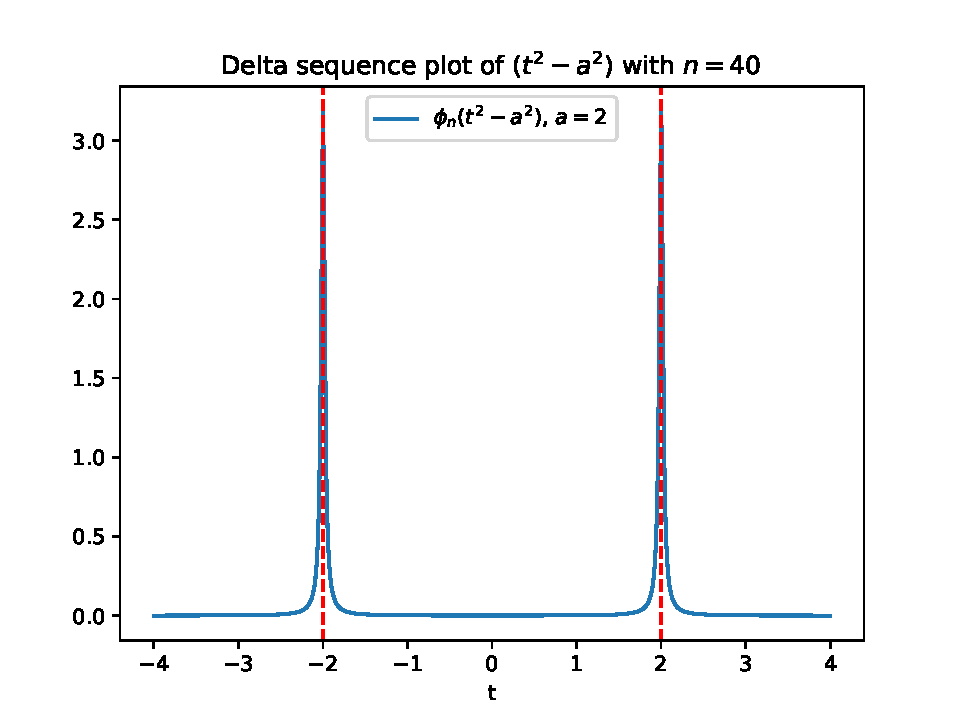
\includegraphics[width=0.6\textwidth]{delta_seq_a.pdf}
    \caption{Delta sequence plot of $\delta[t^2-2^2]$}
    \label{fig:1}
\end{figure}

\begin{figure}[H]
    \centering
    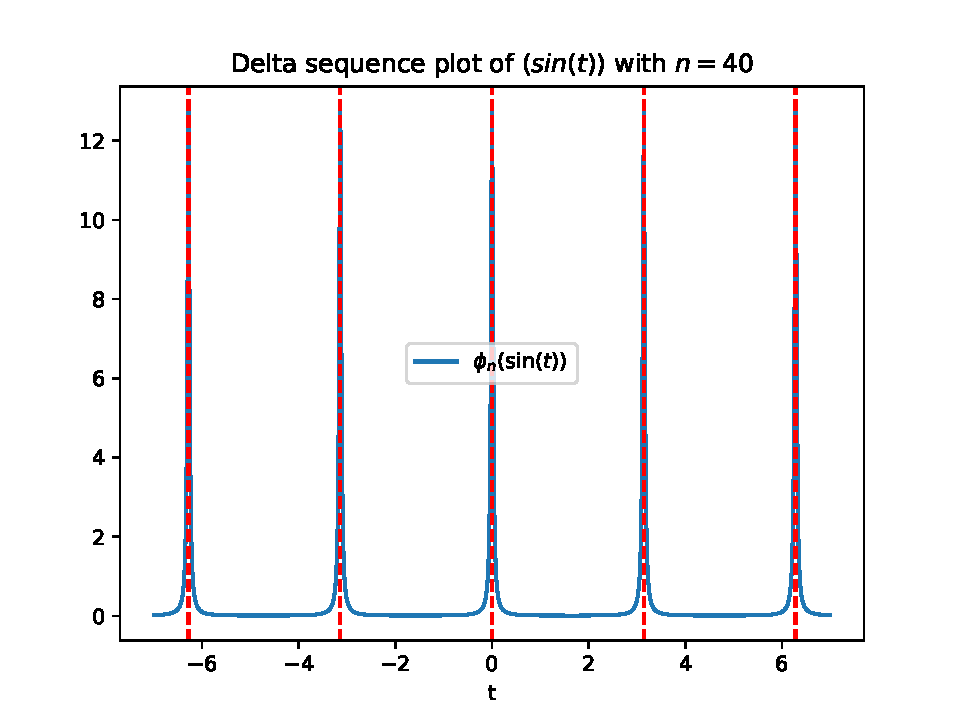
\includegraphics[width=0.6\textwidth]{delta_seq_sin.pdf}
    \caption{Delta sequence plot of $\delta[\sin(t)]$}
    \label{fig:2}
\end{figure}



\subsection*{d)}
Inserting $\delta[\sin(t)]$ from equation \ref{eqn:3b2} gives
\begin{align}
    \int\limits_{-\pi/2}^{\pi/2} \cos(t)\delta[\sin(t)]\dd{t} = \int\limits_{-\pi/2}^{\pi/2}\qty[ \cos(t)\sum_{i=-\infty}^{\infty} \delta[t-\pi i] \dd{t} ]
\end{align}
Since the integral only runs from $-\pi/2$ to $\pi/2$, the values of the integrand outside these limits are irrelevant. The delta-functions only has values at it's zero-points. The only value of $i$ that makes the delta-function fall inside the limits is $i=0$.\footnote{The two neighbouring values, $i=1$ and $i=-1$ will make the spikes fall at $t=\pi$ and $t=-\pi$, which are both outside the limits.} We can therefore replace the sum by only the single delta function $\delta[t]$.

The integral then becomes
\begin{align}
    = \int\limits_{-\pi/2}^{\pi/2} \cos(t) \delta[t] \dd{t} = \cos(0) = 1
\end{align}


\pagebreak
\section*{Appendix: Code for problem 3c}
\inputminted[frame=single, fontsize=\footnotesize]{Python}{delta_seq.py}


\end{document}